% Based on: Dynamics-Compliant Trajectory Diffusion for Super-Nominal Payload Manipulation (CoRL 2025) paper.

\chapter{Conditional Trajectory Diffusion for Dynamic Manipulation Constraints}
\label{ch:payload}

% Colors for torque visualization in figures (prefixed to avoid xcolor naming conflicts)
\definecolor{payloadpastelred}{HTML}{FF746C}
\definecolor{payloadpink}{HTML}{FF9E99}
\definecolor{payloadgreen}{HTML}{006837}
\definecolor{payloadmidgreen}{HTML}{84CA66}
\definecolor{payloadmid}{HTML}{EFBF04}
\definecolor{payloadmidred}{HTML}{F98E52}
\definecolor{payloadred}{HTML}{A50026}

\section{Introduction}
\label{sec:payload:introduction}

\begin{figure}
  \centering
  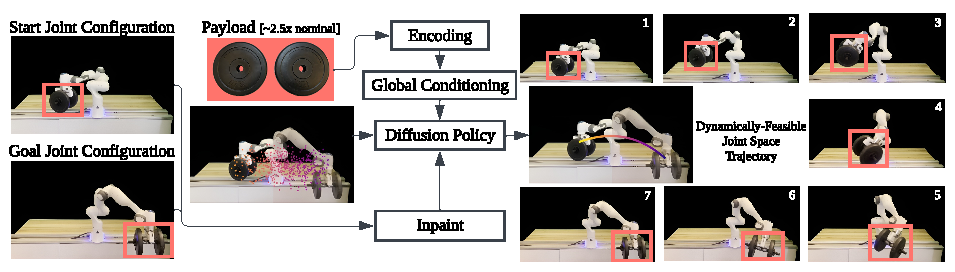
\includegraphics[width=\linewidth]{../payload/graphics/firstnew.pdf}
  \caption{The diffusion model presented in this work learns to generate dynamically feasible trajectories directly in joint angle, velocity, and acceleration space, enabling super-nominal payload manipulation.}\label{payload:fig:firstpg}
\end{figure}

Manipulator design establishes fundamental performance boundaries through the interplay of mechanical structure, actuation system, and control architecture.
At the hardware level, these capabilities manifest as explicit physical constraints: joint angle limits that define the reachable workspace, maximum velocities bounded by motor specifications, and torque limits determined by the drivetrain capacity.
However, a crucial distinction exists between these hardware limitations and the operational capacities specified by manufacturers for general-purpose deployment.
While hardware limits are absolute physical constraints, nominal specifications---like payload capacity and effective workspace boundaries---are \textit{derived} conservatively by considering worst-case scenarios across possible configurations and trajectories.
In practice, system integrators and end-users are locked into treating these derived operational capacities as hard limits rather than contextual capabilities, constrained by warranty requirements to design processes well within these conservative bounds.
This well-established approach of \textit{over-provisioning} hardware to ensure ample safety buffers has system-wide cascading effects---from the need to procure oversized actuators and power supplies, to reinforcing mounting structures for added load tolerance, to expanding facility requirements to accommodate larger equipment.
For instance, when an application requires handling a $35$kg payload, end-users are forced to select a $50$kg-rated robot over a $30$kg-rated system, despite the latter potentially being capable of safely executing the task within broad regions of its operational space.

Importantly, it is possible to overcome the issue of hardware over-provisioning through software-based optimizations, which allow to expand the safe operational envelope of a fixed/given robot embodiment and enable it to perform beyond nominal payload specifications.
This requires unified handling of both geometric (i.e., kinematic) and dynamic constraints, as payload characteristics interact with joint configurations and higher-order derivatives to determine feasible motions.
Even if they have not solved this specific problem, prior approaches in this space have investigated the challenge from multiple perspectives: geometric planners with dynamics post-processing \cite{orthey2023sampling,berscheid2021jerk}, kinodynamic planning \cite{shome2021asymptotically}, optimization-based methods \cite{ichnowski2022gomp}, and control-based frameworks \cite{arrizabalaga2024slosh}. However, these methods face inherent trade-offs between design complexity, constraint handling, and computational efficiency; these become particularly critical when operating near system limits where the feasible solution space becomes highly constrained.
These limitations highlight the need for a method that balances constraint satisfaction with
generalizability---i.e., the ability to adapt to varying payloads, environmental conditions, and task requirements while maintaining consistent performance.

Of note, diffusion models \cite{chi2023diffusionpolicy,sridhar2024nomad} present a compelling opportunity
address the ``curse of dimensionality'' inherent in trajectory planning with simultaneous kinematic and dynamic constraint satisfaction.
\textit{By learning from successful trajectories generated by multiple (imperfect) planning methods}, these models can extract various homotopic solution classes that overcome the limitations of individual approaches.
This distills successful solutions from diverse planning approaches into a unified representation that generalizes across the entire feasible space, including regions where individual planners fail.
The inherent stochasticity in the denoising process enables the exploration of diverse, multimodal trajectories \cite{chi2023diffusionpolicy}, while their capacity to model high-dimensional distributions allows incorporation of rich contextual information such as sensor data and problem constraints.
However, existing diffusion-based approaches have been confined to position-controlled systems \cite{carvalho2023motion,saha2024edmp}, leaving the fundamental challenge of integrating both kinematic and dynamic constraints unaddressed.

In this work, we propose a method that directly tackles this problem by jointly learning valid distributions of positions, velocities, and accelerations that satisfy both constraint types simultaneously---moving beyond prior work that only denoises in position space.
Central to our approach is the use of payload mass---a high-level object property---as a conditioning signal that implicitly encodes the full complexity of payload-induced dynamics into the generative process, without requiring explicit constraint formulation at inference time.
Through investigation of payload encoding strategies, we demonstrate that diffusion models effectively learn the complex relationships between joint states and payload-dependent dynamics, \underline{enabling constant-time generation ($\approx 10$ms) of feasible trajectories that preserve $67.6\%$ workspace accessibility at $3\times$ nominal payload capacity}---without explicit constraint checking at runtime. This demonstrates the importance of dynamics-informed generative models in expanding the operational boundaries of robotic systems.

\section{Related Work}
\label{sec:payload:related}

Manufacturer-specified operational parameters for general deployment of robots are typically far more conservative than hardware-level physical limits and often lack transparency in their derivation.
This has led to significant under-utilization of robotic capabilities, as evidenced by geometric motion planning and time parameterization approaches dominating most industrial use \cite{berscheid2021jerk,coleman2014reducing,orthey2023sampling} and recent advances in foundation models for manipulation in unstructured environments being restricted to exclusively geometric reasoning tasks \cite{o2024open,team2024octo,zitkovich2023rt}.
A nuanced, configuration-dependent understanding of the robot's specifications that considers both robot and environment dynamics could enable a broader spectrum of manipulation capabilities within hardware limits.

Higher-order constraints such as joint torques and end-effector accelerations can be addressed through several approaches that range from ``plan-and-filter'' methods which post-process geometric paths \cite{abderezaei2024clutter,kuntz2019fast} to kinodynamic planners that directly incorporate dynamics during planning \cite{li2015sparse,nayak2022bidirectional,pasricha2024virtues}.
While these approaches offer completeness guarantees, they face practical limitations in high-dimensional manipulation spaces and often exhibit high variance in planning times especially when faced with state or model uncertainty.
These challenges are particularly acute when planning near operational limits, where the feasible solution space becomes increasingly constrained \cite{kingston2018sampling}.
Optimization-based methods naturally accommodate dynamics constraints but rely heavily on good initialization, leading to hybrid approaches that bootstrap the optimization process with learning or sampling-based solutions \cite{ichnowski2020deep,kuntz2019fast,yan2024impact}.
Optimal control formulations for dynamics-aware manipulation also exist \cite{arrizabalaga2024slosh,kim2014catching}. Despite their theoretical rigor, they face practical limitations in handling complex constraints and achieving reliable convergence for real-world manipulation problems.

Importantly, there exist a large body of works that demonstrate how a robot's behavioral repertoire can be significantly expanded when incorporating dynamic constraints---e.g. nonprehensile manipulation \cite{dogar2011framework,pasricha2022pokerrt,ruggiero2018nonprehensile,yu2016more,zeng2020tossingbot} or fast inertial transport \cite{arrizabalaga2024slosh,ichnowski2022gomp,muchacho2022solution,avigal2022gomp}.
These capabilities and considerations are particularly relevant for the specific problem of payload manipulation, where the interaction between payload and induced joint torques significantly influence task success.
Interestingly, payload manipulation presents unique challenges that intersect robot design and control.
Traditionally, prior work has focused on mechanical modeling for specific low-DoF systems \cite{wang2001payload}, with emphasis on payload capacity optimization \cite{korayem2008maximum} and joint torque considerations \cite{nho2003intelligent}. Other work in this domain tackles super-nominal payload handling through the use of multi-arm systems \cite{kim2021enhancing,yan2016coordinated}.
However, the field lacks generalizable approaches for high-DoF systems that can reason about dynamic payload-robot interactions across diverse tasks.

Learning-based approaches offer promising directions for both generalizability and efficient trajectory generation in high-dimensional constrained spaces while respecting system dynamics. Autoregressive models implicitly encode dynamics through dataset design \cite{fishman2023motion,qureshi2020motion}, while recent diffusion-based approaches provide non-autoregressive alternatives with improved sampling diversity \cite{carvalho2023motion,saha2024edmp}. Task-level diffusion policies, conditioned on language and visual embeddings \cite{ajay2023is,chi2023diffusionpolicy}, demonstrate potential for generating diverse behaviors from high-level task specifications.
Our method conditions a denoising diffusion model on the target payload to generate dynamically feasible trajectories.

\section{Diffusion Models for Trajectory Generation}
\label{payload:sec:diffusion}

Diffusion models are a class of generative models that produce high-quality and diverse samples across multiple data modalities \cite{ho2020denoising}.
These models operate through a two-phase process: first, gradually corrupting training data with Gaussian noise in a forward process, then learning to reverse this corruption through an iterative denoising process.
In the context of robot motion planning, we use diffusion to generate collision-free and dynamically feasible trajectories.

A joint space trajectory with $t$ waypoints at denoising step $k$ is defined as
$\bm{\pi}^k = [ X_0^k, X_1^k, \dots, X_{t-1}^k ]^T$
where $X_i = (q_i, \dot{q}_i, \ddot{q}_i) \in \mathbb{R}^{3n}$ represents the complete state (joint angles, velocities, and accelerations) of an $n$-DoF robot arm at timestep $i$.
The training process for the diffusion model approximates the conditional distribution $p(\bm{\pi}\ |\ \mathcal{P})$, where $\mathcal{P}$ is the target payload representation (\Cref{payload:sec:model}).
It does so by sampling $\bm{\pi}$ from dataset $\mathcal{D}$, adding noise according to a noise schedule parameterized by $\alpha$, $\gamma$, and $\sigma$, and learning to predict the underlying sample. The noise prediction network $\epsilon_\theta$, where $\theta$ represents the parameters of the 1D U-Net architecture, is trained to minimize
    $\mathcal{L}(\theta) = MSE(\epsilon^k, \epsilon_\theta(\mathcal{P}, \bm{\pi}^0 + \epsilon^k, k))$.

Given a trained $\epsilon_\theta$, the $K$-step iterative denoising process
    $\bm{\pi}^{k-1} = \alpha \cdot (\bm{\pi}^k - \gamma\epsilon_\theta(\mathcal{P}, \bm{\pi}^k, k) + \mathcal{N}(0, \sigma^2I))$
starts from $\bm{\pi}^K \sim \mathcal{N}(0, I)$ and generates a trajectory $\bm{\pi}^0$ that can support a target payload and obeys start, goal, joint limit, and collision constraints.
In practice, start and goal states are enforced via inpainting \cite{carvalho2023motion}, i.e., $\bm{\pi}_0^k = X_{start}$ and $\bm{\pi}_{t-1}^k = X_{goal}$ where $\dot{q}_{start} = \dot{q}_{goal} = \ddot{q}_{start} = \ddot{q}_{goal} = \bm{0}$.
Collisions are avoided via inference-time gradient guidance $\bm{\pi}^{k-1} = \bm{\pi}^k - \beta\ \cdot \nabla J(\bm{\pi}; E)$ where $\beta$ is a tunable guidance weight, $J$ defines the collision cost function, and $E$ represents the set of all obstacles in the environment \cite{saha2024edmp}.
Additionally, joint limits are enforced via clamping during the training and inference processes.
Specific to our work, $p(\bm{\pi}\ |\ \mathcal{P})$ implicitly models dynamically feasible payload-induced torques through an object property-based global conditioning mechanism that influences the entire trajectory by appending target payload representation $m$ to the diffusion timestep embedding in the noise prediction network architecture \cite{chi2023diffusionpolicy}.

\section{Payload-Conditioned Trajectory Denoising}
\label{sec:payload:denoising}

In this section, we present our payload-conditioned diffusion model to generate pick-and-place trajectories that transport super-nominal payloads while obeying kinematic and dynamic constraints.

\subsection{Training Data}

Our payload-conditioned diffusion model (\Cref{payload:sec:model}) is trained on $25,000$ time-parameterized, collision-free joint space trajectories (state dimension = DoF$\times3$, corresponding to joint angles, velocities, and accelerations) for tabletop pick-and-place motions. These trajectories are generated using a plan-and-filter pipeline that uses cuRobo, a GPU-accelerated trajectory optimization framework \cite{sundaralingam2023curobo}, followed by a dynamics validation step (\Cref{payload:fig:data-generation}).

\begin{wrapfigure}{r}{0.5\textwidth}
  \centering
  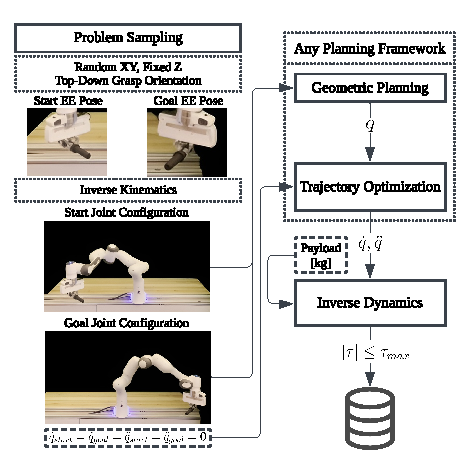
\includegraphics[width=\linewidth]{../payload/graphics/datagen.pdf}
  \caption{Plan-and-filter process to create training data.}
  \label{payload:fig:data-generation}
\end{wrapfigure}

First, trajectories are generated for the 7DoF Franka Emika Panda robot arm with an effective payload mass of $0$kg.
Second, to ensure that payload-induced joint torques remain within hardware limits, each trajectory is verified through an analytically-derived dynamics model parameterized on real-world data \cite{gaz2019dynamic}.
This model captures both the standard dynamic elements (inertia, Coriolis, and gravity) and velocity-dependent joint friction.
By using a dynamics model fitted to real robot trajectory data, we ensure that our training dataset reflects the physical constraints observed in hardware.

This dynamics verification step utilizes a complete robot model where $q$, $\dot{q}$, $\ddot{q}$, and $\tau$ are $7\times1$ vectors representing joint angles, velocities, accelerations, and torques respectively.
The dynamics matrices include: $M(q)$ ($7\times7$ positive-definite, symmetric joint inertia matrix), $C(q,\dot{q})$ ($7\times7$ Coriolis/centrifugal matrix), $g(q)$ ($7\times1$ gravity compensation torque vector), and $f(\dot{q})$ ($7\times1$ joint friction torque vector). External task space forces $F_{ext}$ ($6\times1$) map to joint torques through the Jacobian $J(q)$ ($7\times7$).
The dynamics model is parameterized as:
\begin{equation}\label{payload:eq:arm-dyns}
    \tau = M(q)\ddot{q} + C(q, \dot{q})\dot{q} + g(q) + f(\dot{q}) + J^{-1}(q)F_{ext}
\end{equation}
Note that this analytically-derived model represents the robot without external payloads which can affect model accuracy when considering varying payload masses in real-world deployment.
To account for payload-induced joint torques, we model the gravitational effects as a 6D Cartesian wrench transformed from the world frame to the end-effector frame.
This frame transformation is critical for accurately projecting gravitational forces acting on the payload along the robot's embodiment.
We represent the external gravitational wrench $\bm{F}_g \in \mathbb{R}^6$ in the world frame with a simplified point mass model:
$\bm{F}_g = mg \cdot [0,\ 0,\ -1,\ 0,\ 0,\ 0]^T$
where $m \in \mathbb{R}^+$ denotes payload mass and $g \approx 9.81 \text{ m/s}^2$ is gravitational acceleration. This representation assumes force application at the object's center of mass, neglecting potential moment contributions.
The wrench's structure combines linear forces (first three components) and angular forces (last three components), which are
mapped to induced joint torques through the manipulator Jacobian, contributing to the total joint torque vector (\cref{payload:eq:arm-dyns}).

The training dataset $\mathcal{D}$ is constructed from these trajectories that satisfy both kinematic and dynamic constraints. Each element $d_i \in \mathcal{D}$ is a tuple of trajectory $\bm{\pi}_i$ and maximum supported payload $m_i$.
Each $m_i$ is the maximum supported payload mass for trajectory $i$ subject to $|\tau(\bm{\pi}_i, m_i)| \leq \tau_{max}$, $\forall t \in [0,T]$ where $\tau_t$ is computed via the dynamics equation (\cref{payload:eq:arm-dyns}).

Having established our dataset $\mathcal{D}$ of dynamically feasible trajectories and their corresponding maximum payload limits, we now consider different ways of incorporating payload conditioning into the diffusion model architecture.

\subsection{Payload-Conditional Trajectory Generation}
\label{payload:sec:model}

We extend the diffusion policy architecture to condition trajectory generation on payload mass through global conditioning \cite{chi2023diffusionpolicy}. Unlike local conditioning where features influence each waypoint individually, global conditioning applies the mass embedding uniformly across the entire trajectory generation process, preserving dynamic feasibility across the generated motion (\Cref{payload:fig:architecture}).

\begin{wrapfigure}{l}{0.48\textwidth}
  \centering
  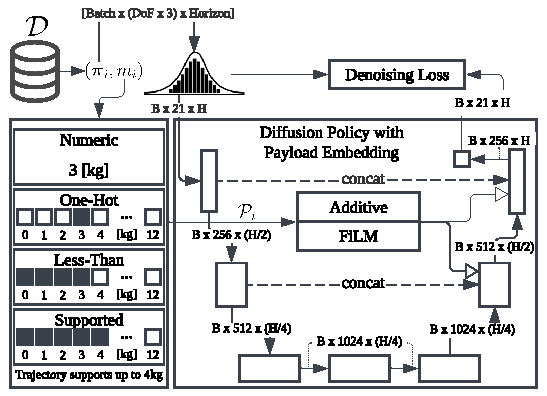
\includegraphics[width=\linewidth]{../payload/graphics/archnew.pdf}
  \caption{Our model conditions a 1D UNet denoising architecture \cite{chi2023diffusionpolicy} on various payload embeddings.}
  \label{payload:fig:architecture}
\end{wrapfigure}

For each training trajectory $i$ with corresponding maximum supported payload mass $m_i \in \mathcal{D}$, we investigate four approaches to incorporate a target payload mass $p_i$ into an encoding vector $\mathcal{P}_i$.
The payload encoding $\mathcal{P}$ is concatenated with a diffusion timestep embedding to form a global conditioning vector, which is then integrated into $\epsilon_\theta$ through either additive or affine transform conditioning \cite{perez2018film}.
We consider the following approaches for designing $\mathcal{P}$.

\noindent\textbf{Numeric Input.} A random supported mass scalar $p_i \sim \mathcal{U}(0, m_i)$ is sampled and fed directly to the network. This approach naturally supports continuous payload values during inference, despite training on a discrete set of payload values.

\noindent\textbf{One-Hot Encoding.} For a system supporting payloads from $0-18$kg in $1$kg increments, a random supported mass $p_i \sim \mathcal{U}(0, m_i)$ is encoded as a $19$-dimensional binary vector with a single non-zero entry at index $\lceil p_i \rceil$.
While this categorical representation simplifies the learning task by discretizing the payload space, it constrains inference to the discrete payload values seen during training.
During inference, continuous payload masses must be quantized to their ceiling value $\lceil p \rceil$ before input to the denoising network, ensuring a tight upper bound for conservative operation.

\noindent\textbf{Less-Than Encoding.} This encoding exploits the logical constraint that trajectories supporting a given payload must also support all lighter payloads.
For a random supported mass $p_i \sim \mathcal{U}(0, m_i)$, we construct a $19$-dimensional binary vector where entries are $1$ for indices $j \leq \lceil p_i \rceil$ and $0$ otherwise.
This representation directly encodes the downward compatibility constraint into the input space, potentially improving the network's ability to learn and respect payload-dependent constraints.
During inference, continuous payload masses are similarly mapped to their ceiling value $\lceil p \rceil$ to construct the binary encoding.

\noindent\textbf{Supported-Range Encoding.}
This approach encodes the complete range of supported payloads for a given trajectory.
For training trajectory $i$ with maximum supported mass $m_i$, we construct a $19$-dimensional binary vector where entries are $1$ for indices $j \leq \lceil m_i \rceil$ and $0$ otherwise.
During training, this encoding preserves the full payload compatibility information from $\mathcal{D}$.
At inference time, for a target payload mass $p$, the encoding can be constructed either as a one-hot vector with a single non-zero entry at index $\lceil p \rceil$, or as a less-than encoding with ones for indices $j \leq \lceil p \rceil$.
This dual interpretation enables both trajectory generation for specific payloads and exploration of the learned manifold of payload-trajectory relationships.
Broadly, each encoding method presents trade-offs between generalization capability and training simplicity.

\section{Evaluation}
\label{sec:payload:evaluation}

To validate our method, we focus on pick-and-place motions---a canonical industrial robotics requirement where super-nominal payload manipulation can significantly extend the operational envelope of robot arms while obeying strict hardware limits.\footnote{Please refer to the supplementary material for more details on compute hardware, problem domain, experimental setup, and baseline methods. Videos are available here: \url{https://payload-diffusion.github.io/}}
In our experiments, payloads were rigidly attached to the end-effector with a geometrically centered and uniform mass distribution. This was a deliberate experimental choice necessitated by the limited grasping force of our parallel gripper, ensuring repeatable execution across trials. Importantly, this choice is not a fundamental limitation of our method: as shown in the supplementary video, our approach is capable of handling non-rigidly attached objects and payloads with modest center-of-mass offsets, though some failure modes at higher payloads are also highlighted and explained there.
During execution, invalid trajectories generated by the diffusion model are simply not executed. For valid trajectories that fail due to unmodeled dynamics (e.g., payload oscillations), standard robot safety stops are triggered automatically. Our approach relies on the manufacturer's joint velocity controller for trajectory tracking, which provides sufficiently accurate state tracking for the tasks evaluated in this work.

\subsection{Comparison of Payload Encodings}

Our evaluation of different payload encodings, conducted with FiLM conditioning and payload encoding normalization, reveals several key insights in terms of planning success rate (\Cref{payload:fig:bar}).

\begin{wrapfigure}{r}{0.6\textwidth}
  \centering
  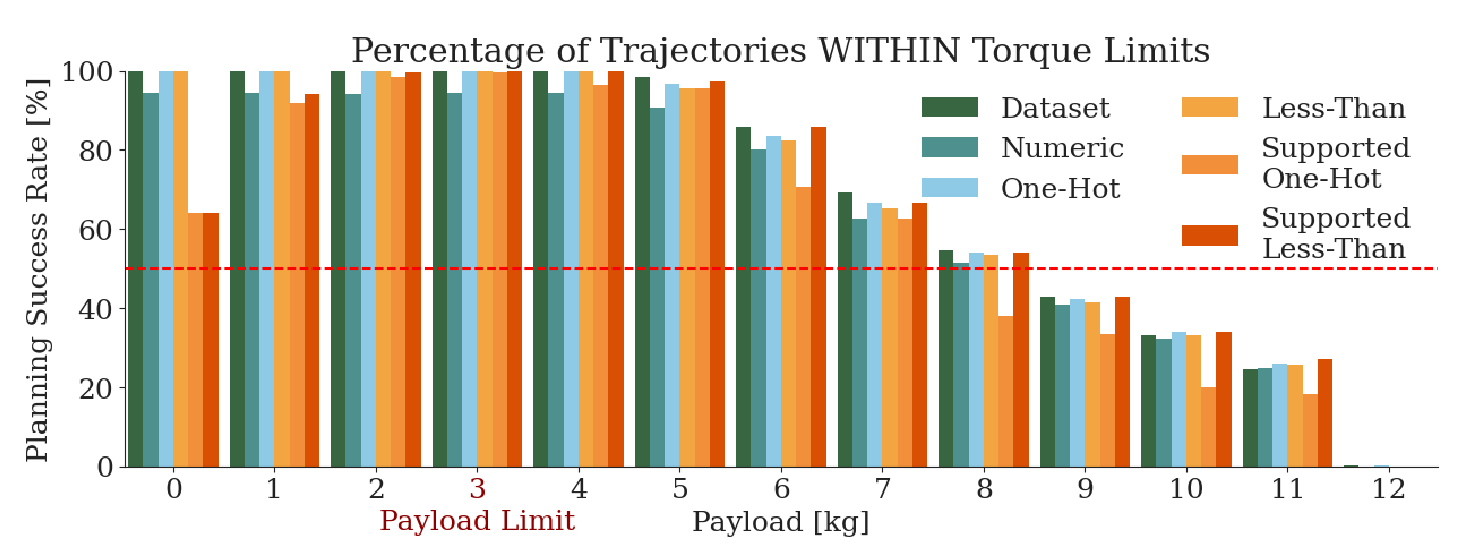
\includegraphics[width=\linewidth]{../payload/graphics/bar.pdf}
  \caption{The aggregate success rate metric shows one-hot diffusion closely matching the underlying training data distribution.}\label{payload:fig:bar}
\end{wrapfigure}

Numeric and one-hot approaches demonstrate comparable effectiveness, particularly for payloads within nominal capacity ($0-3$kg). However, all methods show a tendency to underestimate success rates for higher payloads, potentially due to data imbalance in the training set. When interpreted as a less-than encoding during inference, the supported-range encoding achieves competitive performance, but its one-hot interpretation leads to significantly lower success rates.
While the encoding is designed to capture richer payload-trajectory relationships, the network struggles to fully utilize this information during generation.
The inability of numeric, supported one-hot, and supported less-than encodings to achieve $100\%$ success rates in the most loosely-constrained and data-rich portions of the state space, i.e., the nominal operating regime ($0-3$ kg), suggest fundamental limitations in how these encoding schemes enable the diffusion model to obey kinematic and dynamic constraints.
For subsequent experiments, we use with the one-hot encoding scheme, which demonstrates superior performance in terms of success rate.

\begin{figure}
  \centering
  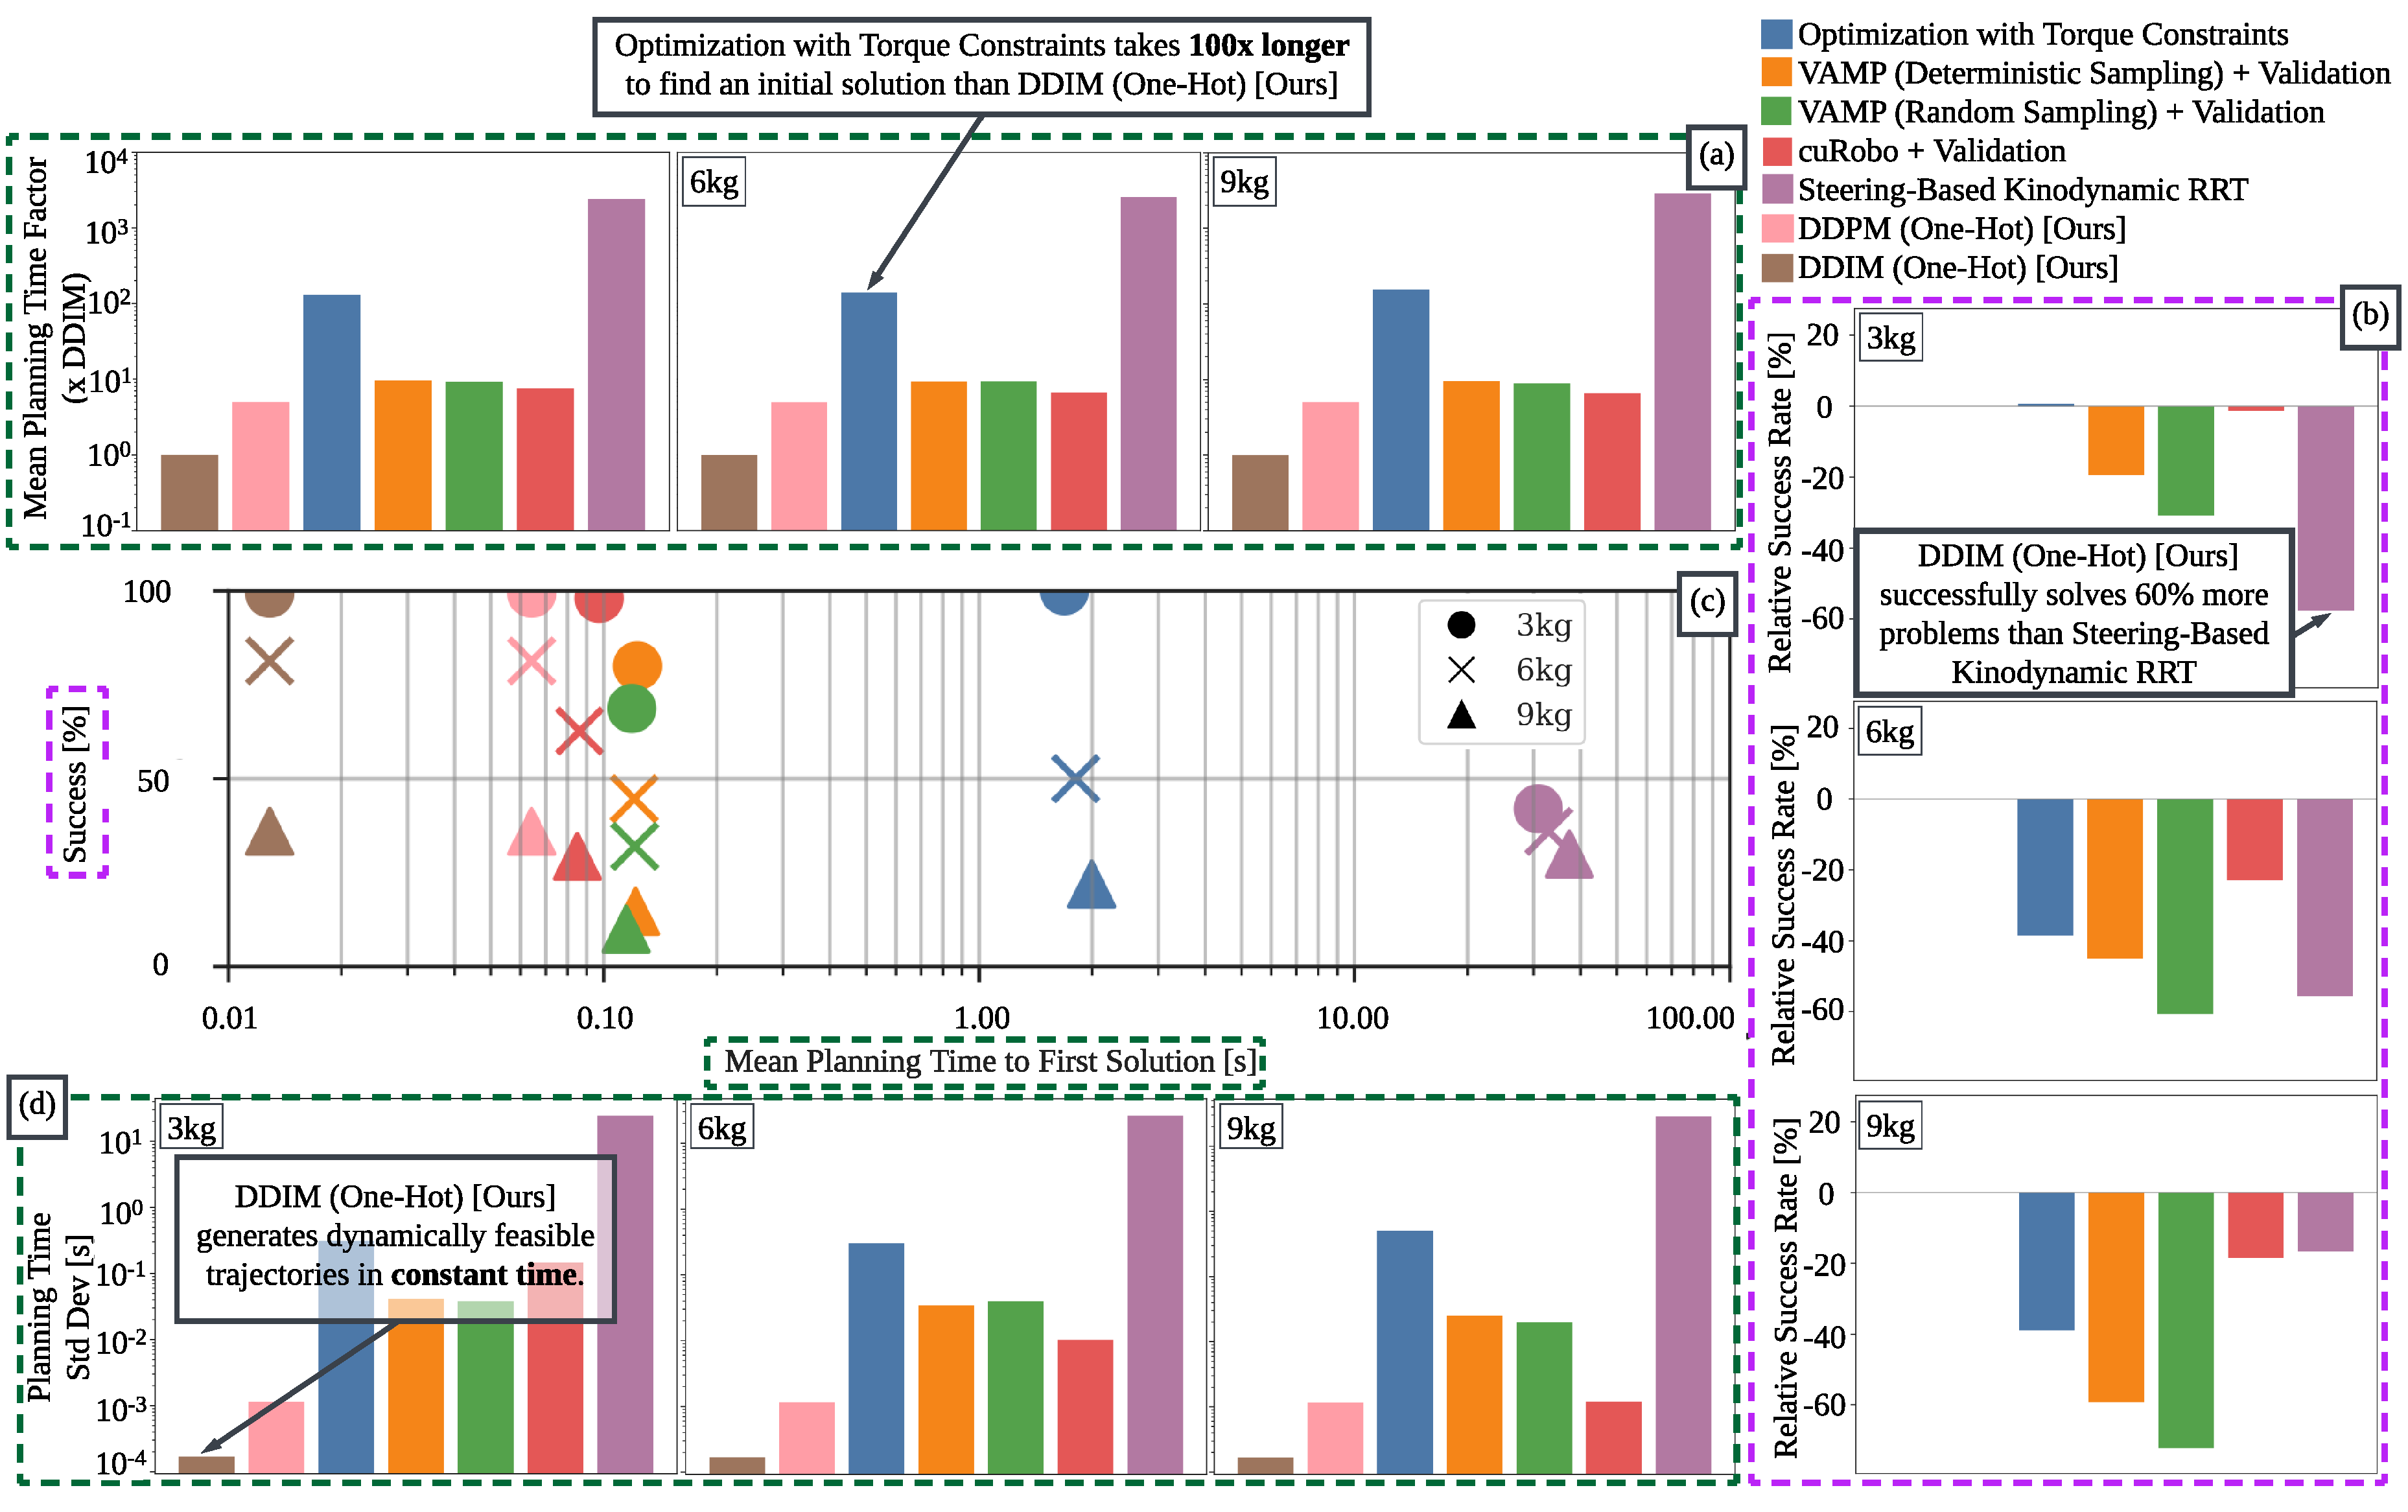
\includegraphics[width=\linewidth]{../payload/graphics/eval.pdf}
  \caption{Comparative analysis of trajectory planning methods for payloads of $3$kg, $6$kg, and $9$kg. DDIM (One-Hot) significantly outperforms a variety of baseline methods in both planning time to first solution and success rate, generating dynamically feasible trajectories in constant time across all payload conditions.}\label{payload:fig:eval}
\end{figure}

\subsection{Comparison across Planner Types}

For the purposes of our discussion, we refer to DDIM (One-Hot) as a primary point of comparison. Denoising Diffusion Implicit Models (DDIM) offer accelerated inference due to fewer denoising steps (in our case, $5$) \cite{song2021denoising}. We also present results for DDPM \cite{ho2020denoising} with $25$ denoising steps. Notably, our experiments demonstrate that DDIM achieves identical success rates to DDPM despite requiring significantly less planning time ($\approx 0.01$s), validating our approach for realtime use (\Cref{payload:fig:eval}c).

We evaluate our approach against a diverse set of trajectory planning methods using mean planning time to first solution and the corresponding success rate over $500$ tabletop manipulation tasks as the primary metric (\Cref{payload:fig:eval}c). This metric provides a fair basis for comparison across fundamentally different planning paradigms. Additional metrics include planning time factor (mean planning time of baseline / mean planning time of DDIM) (\Cref{payload:fig:eval}a), relative success rate change over DDIM as a percentage (\Cref{payload:fig:eval}b), and standard deviations of planning times (\Cref{payload:fig:eval}d).

\paragraph{Plan-and-Filter Methods}

Broadly, plan-and-filter methods employ a sequential process: first planning a geometric path via sampling-based motion planning, then time-parameterizing it to derive joint velocities and accelerations, and finally validating trajectory feasibility for the target payload using the robot dynamics model (\cref{payload:eq:arm-dyns}).
This iterative process continues until a feasible trajectory is found that satisfies all joint torque constraints induced by the payload \cite{abderezaei2024clutter}.
We evaluate two CPU-accelerated geometric planning variants: VAMP (RRTConnect) with deterministic sampling and VAMP (RRTConnect) with random sampling \cite{thomason2024motions}. We select Ruckig for time parameterization due to its ability to generate time-optimal trajectories in realtime \cite{berscheid2021jerk}.
Geometric motion planning and time parameterization can alternatively be unified within a single optimization framework (in our case, cuRobo) which can be followed by the dynamics validity checking.

Since there is a decoupling between kinematic reasoning and dynamic reasoning, further exacerbated by the separate time parameterization step in the VAMP variants, these approaches demonstrate inferior performance compared to our one-hot DDIM model (Fig.~\ref{payload:fig:eval}c).
VAMP with deterministic sampling achieves marginally higher success rates than VAMP with random sampling due to its low-dispersion sampling strategy, which provides more uniform exploration of the configuration space.
Despite this sampling advantage, both variants exhibit higher standard deviations (Fig.~\ref{payload:fig:eval}d) and lower overall success rates, particularly with heavier payloads (Fig.~\ref{payload:fig:eval}b). These methods also exhibit significant planning time variability (Fig.~\ref{payload:fig:eval}a).
The temporal predictability of our approach is particularly valuable for industrial pipelines, where high standard deviations in planning times can complicate integration with broader automation workflows.
The success rate differential between cuRobo and DDIM particularly demonstrates that our model effectively learns from successful trajectories generated by imperfect planners. While cuRobo with validation often requires multiple attempts to find feasible solutions, our method leverages these curated trajectories during training to achieve higher success rates, especially under super-nominal payload conditions.

\paragraph{Kinodynamic Motion Planning}

Plan-and-filter methods generate paths requiring post-processing to satisfy dynamic constraints, potentially invalidating the solution. By planning directly in the state space that includes joint angles, velocities and accelerations, kinodynamic planning ensures dynamically feasible solutions from the outset.
Specifically, we employ steering-based kinodynamic RRT as our baseline, planning in the joint angle, velocity, and acceleration space \cite{lavalle2001randomized}. Ruckig serves as our steering function owing to its ability to operate in realtime while respecting third-order constraints \cite{berscheid2021jerk}. Each edge undergoes validity checking that includes dynamics (\cref{payload:eq:arm-dyns}) and smoothness checks before addition to the planning graph.
Results not only indicate high planning times to find the first solution ($>1000\times$ compared to DDIM) due to ``the curse of dimensionality'' (\Cref{payload:fig:eval}a), but also show high standard deviations due to random sampling in the high-dimensional state space (\Cref{payload:fig:eval}d).
The clustering of success rates observed across all three payloads suggests an inherent planning bias in kinodynamic RRT, indicating insufficient exploration in this highly non-Euclidean state space (\Cref{payload:fig:eval}a).
Furthermore, kinodynamic approaches require extensive tuning of hyperparameters that interact with system dynamics in complex ways. Suboptimal parameter selection frequently results in planning timeouts or physically implausible trajectories.

\paragraph{Trajectory Optimization with Torque Constraints}

This baseline implements Sequential Least SQuares Programming (SLSQP) optimization for trajectory generation, minimizing sum-squared jerk to ensure smoothness \cite{ichnowski2022gomp}. To facilitate direct comparison with our method, we constrain trajectory durations instead of performing time optimization \cite{sundaralingam2023curobo,ichnowski2022gomp}, isolating evaluation to payload manipulation capabilities. The formulation incorporates linearized representations of both dynamic payload constraints and collision avoidance parameters.
The success rate disparity between optimization and DDIM becomes particularly pronounced with higher payloads as the optimization landscape becomes increasingly constrained.
This significant performance gap warrants discussion in the context of our evaluation choices. We implemented a basic SLSQP optimization formulation to establish a baseline that directly handles dynamic constraints without sophisticated warm-starting or acceleration techniques. Recent work has shown that optimization-based planners can achieve substantially better performance both in planning time and success rate through strategies like learning-based seeding \cite{ichnowski2020deep,huang2024diffusionseeder}.
However, our baseline still highlights the computational challenge of finding feasible solutions in high-dimensional spaces with nonlinear dynamic constraints.

\begin{figure}
  \centering
  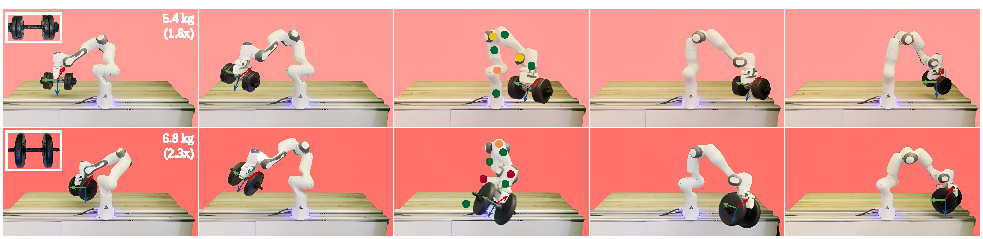
\includegraphics[width=\linewidth]{../payload/graphics/vignew.pdf}
  \caption{Two qualitative motions of the robot carrying super-nominal payloads of \textcolor{payloadpink}{$5.4$kg ($1.8\times$ nominal capacity)} and \textcolor{payloadpastelred}{$6.8$kg ($2.3\times$ nominal capacity)} are shown. Colored dots indicate joint torques as a percentage of joint limits: \textcolor{payloadgreen}{$0-20\%$}, \textcolor{payloadmidgreen}{$20-40\%$}, \textcolor{payloadmid}{$40-60\%$}, \textcolor{payloadmidred}{$60-80\%$}, \textcolor{payloadred}{$80-100\%$}. Joints 1, 3, and 5 exhibit higher torques, with joint 1 bearing the structural load of the arm and joints 3 and 5 positioning and orienting the payload.}\label{payload:fig:vignette}
\end{figure}

\section{Conclusion}
\label{sec:payload:conclusion}

This work demonstrates that manipulators can safely operate well beyond their nominal payload ratings through diffusion-based trajectory generation, challenging the traditional approach of hardware over-provisioning in industrial automation.
By training on trajectories that span the full range of payload-dependent dynamic constraints and leveraging the successes of ``imperfect'' planners, our model learns to generate motions for complex tasks in constant time that naturally respect system limitations without explicit constraint checking at runtime. This enables safe operation even at super-nominal payloads, maintaining $67.6\%$ of the nominal workspace at $3\times$ rated capacity.\footnote{More details on accessible workspace regions in the supplementary material.}

Potential avenues for future work include studying how to determine the optimal composition of training data from different planners operating in varied environments.
Moreover, the notion of conditioning on object-level characteristics can be generalized to handle objects with internal dynamics like liquids or articulated parts, moving beyond rigid-body assumptions.
Such a framework could significantly reduce robotic system integration complexity and design burden by eliminating separate subsystems for different planning aspects, while maintaining the computational efficiency advantages and higher-order constraint satisfaction demonstrated in this work.

\section{Limitations}
\label{sec:payload:limitations}

While our results establish the viability of super-nominal payload manipulation on fixed/given hardware, several aspects warrant further discussion. \textbf{Rigid Attachment Choice.} Even though the rigid attachment experimental choice simplifies analysis by eliminating offset moments, it introduces two critical limitations in real-world execution (see accompanying video): dynamic effects from payload oscillation when objects are not perfectly rigid, and unmodeled torques when the object's center of mass is significantly offset from the end-effector's origin. These assumptions can lead to trajectory tracking errors or even task failures, particularly when handling flexible materials or asymmetric objects. Looking ahead, extending our approach to objects with internal dynamics will require explicit robot-object dynamics models to capture effects such as rotational inertia, slippage, and uneven mass distributions. Incorporating these nonlinearities, together with friction modeling for fingered grippers and suction force modeling for suction-based end-effectors, remains an important direction. Moreover, expanding the conditioning space to whole-body contact forces, fingertip wrench cones, and suction dynamics, as well as embedding more advanced controllers (e.g., impedance or admittance), will allow the same ``constraint-aware by design'' principle to scale to interaction-rich manipulation tasks. \textbf{Test-Time Robustness.} Assessing test-time robustness requires long-term deployment studies and, in many cases, proprietary Original Equipment Manufacturer (OEM) data on wear-and-tear. Whether robots should operate continuously at or near maximum capacity is also a design question for robot OEMs. While our method generates trajectories that respect manufacturer-specified torque limits, joints do run hotter under high payloads, motivating further study of safety margins under sustained operation. \textbf{Embodiment Generalization.} We acknowledge that embodiment understanding must be more directly incorporated into the training process to enable generalization across different robotic platforms. To this end, we are developing more general embodiment-constrained conditioning mechanisms as part of ongoing work.

Our work also raises important theoretical questions about completeness and optimality guarantees for learning-based motion planning. Even though we can argue that diffusion models trained on optimal trajectories will generate similarly optimal solutions, establishing formal completeness guarantees remains an open challenge.
Moreover, while our method demonstrates advantages in inference speed, traditional optimization-based approaches offer clearer constraint satisfaction guarantees and greater flexibility in adapting to new constraints without retraining. That said, training is not a bottleneck: we generate training trajectories across multiple payload conditions, with each trajectory verified for kinematic and dynamic feasibility throughout the robot's operational workspace. The compact dimensionality of our denoised samples enables fast retraining of the UNet and efficient creation of a high-quality dataset with comprehensive operational space coverage, but without the need for real-world payload manipulation data (assuming the existence of a robot dynamics model, which also lends to system modularity).

More rigorous evaluations comparing CPU versus GPU performance and Python versus C++ implementations would enable direct baseline comparisons but standardizing these benchmarks remains challenging. Our evaluation of baseline methods maintains industry-standard implementations of baselines without additional optimizations for deployment infrastructure.
Several other under-explored areas of research remain: optimal training data selection for maximizing planner generalization, disambiguating data imbalance from model generalization to explain the high variance in torques for higher payloads, leveraging diffusion models' continual learning capabilities at industrial scale, and conditioning on real-world sensor modalities like point clouds for deployment.

\section{Case Study: Diffusion Under Failure-Induced Embodiments}
\label{ch:failures}

\subsection{Motivation}
\label{sec:failures:revisit}

The Mars rover Opportunity's robotic arm first stalled on November 25, 2005; its shoulder joint experienced intermittent motor stalls for years, managed with voltage workarounds and revised stow procedures. Similarly, Curiosity's drill paused sampling for roughly eighteen months until a hand-designed drilling method restored coring \cite{nasa_science_first_drilled_sample_2018,jpl_opportunity_shoulder_2008}. Cases like these underscore that failures in continuously operating systems are inevitable \cite{factory_efficiency_2020}. Prevailing safety standards mandate \textsl{fail-freeze} behavior, requiring robots to halt when faults are detected \cite{ISO10218-1,ISO13849-1,IEC60204-1}. The result is prolonged downtime and reduced autonomy.
In this work, we contrast this overly conservative approach with \textsl{fail-active} behavior, a more ambitious (and harder to achieve) reliability goal in which robots maintain functionality, full or reduced, under fault conditions \cite{aero_reliability}. \textbf{Fail-active behavior is how humans operate}: we continue walking on a sprained ankle, writing with a non-dominant hand, going to work when we've had our hearts broken.

Faults reshape what the robot can physically do: actuation failures (e.g., joint range and velocity restrictions) shrink the feasible workspace and degrade manipulability, electrical faults (e.g., brownouts) reduce control authority, sensor drift can distort state estimates, and end-effector wear (e.g. lowered friction) degrades contact mechanics. Ultimately, these physical changes mean the robot can no longer move the way it originally planned.

In this case study, we focus on \textit{actuation failures} as they directly affect how the robot moves. \textit{Fail-active} operation requires adapting to these altered kinematics, which can cause end-effector motion to become non-holonomic; meaning the same control input may no longer yield the same end-effector motion \cite{Bloch_Krishnaprasad_Murray_2016}.
It is also important to note that since degradation can evolve over time \cite{barbieri2015sensor} and the failure state is not known a priori, \textbf{the space of failure modes is effectively unbounded}. Moreover, each joint can fail independently in multiple ways, and this complexity scales combinatorially with the robot's degrees of freedom, \textbf{making reliable performance across failures hard to engineer}.

As failure-induced constraints redefine the robot's workspace, manipulability, and feasible interactions with the world, \textsl{we posit that each failure mode can be interpreted as a new embodiment}.
Through this lens, different embodiments are unable to perform the same tasks using the same behaviors. As no same set of behaviors can span all embodiments, multiple motion primitives are needed to expand the feasible action space and reachable task-space \cite{briscoe2024exploring}.

Synthesizing effective motion primitives for arbitrary failure conditions is challenging due to the complex relationship between robot embodiment constraints and feasible task-space behaviors. Existing approaches fall short in three key gaps: 1) they do not generalize to arbitrary failure configurations \cite{briscoe2024exploring,xie2021maximizing}; 2) they are not capable of completing multiple manipulation primitives \cite{pham2024adaptive}; and 3) they do not address multi-joint failures \cite{mu2016kinematic,kim2024quadrupedal}. To the best of the authors' knowledge, no existing work bridges all three of these gaps simultaneously.
Diffusion models are uniquely suited to solve this. Because they excel at modeling multimodal data distributions, diffusion policies can generate across the range of actions required to span these infinite embodiments at inference.

\begin{figure}
    \centering
    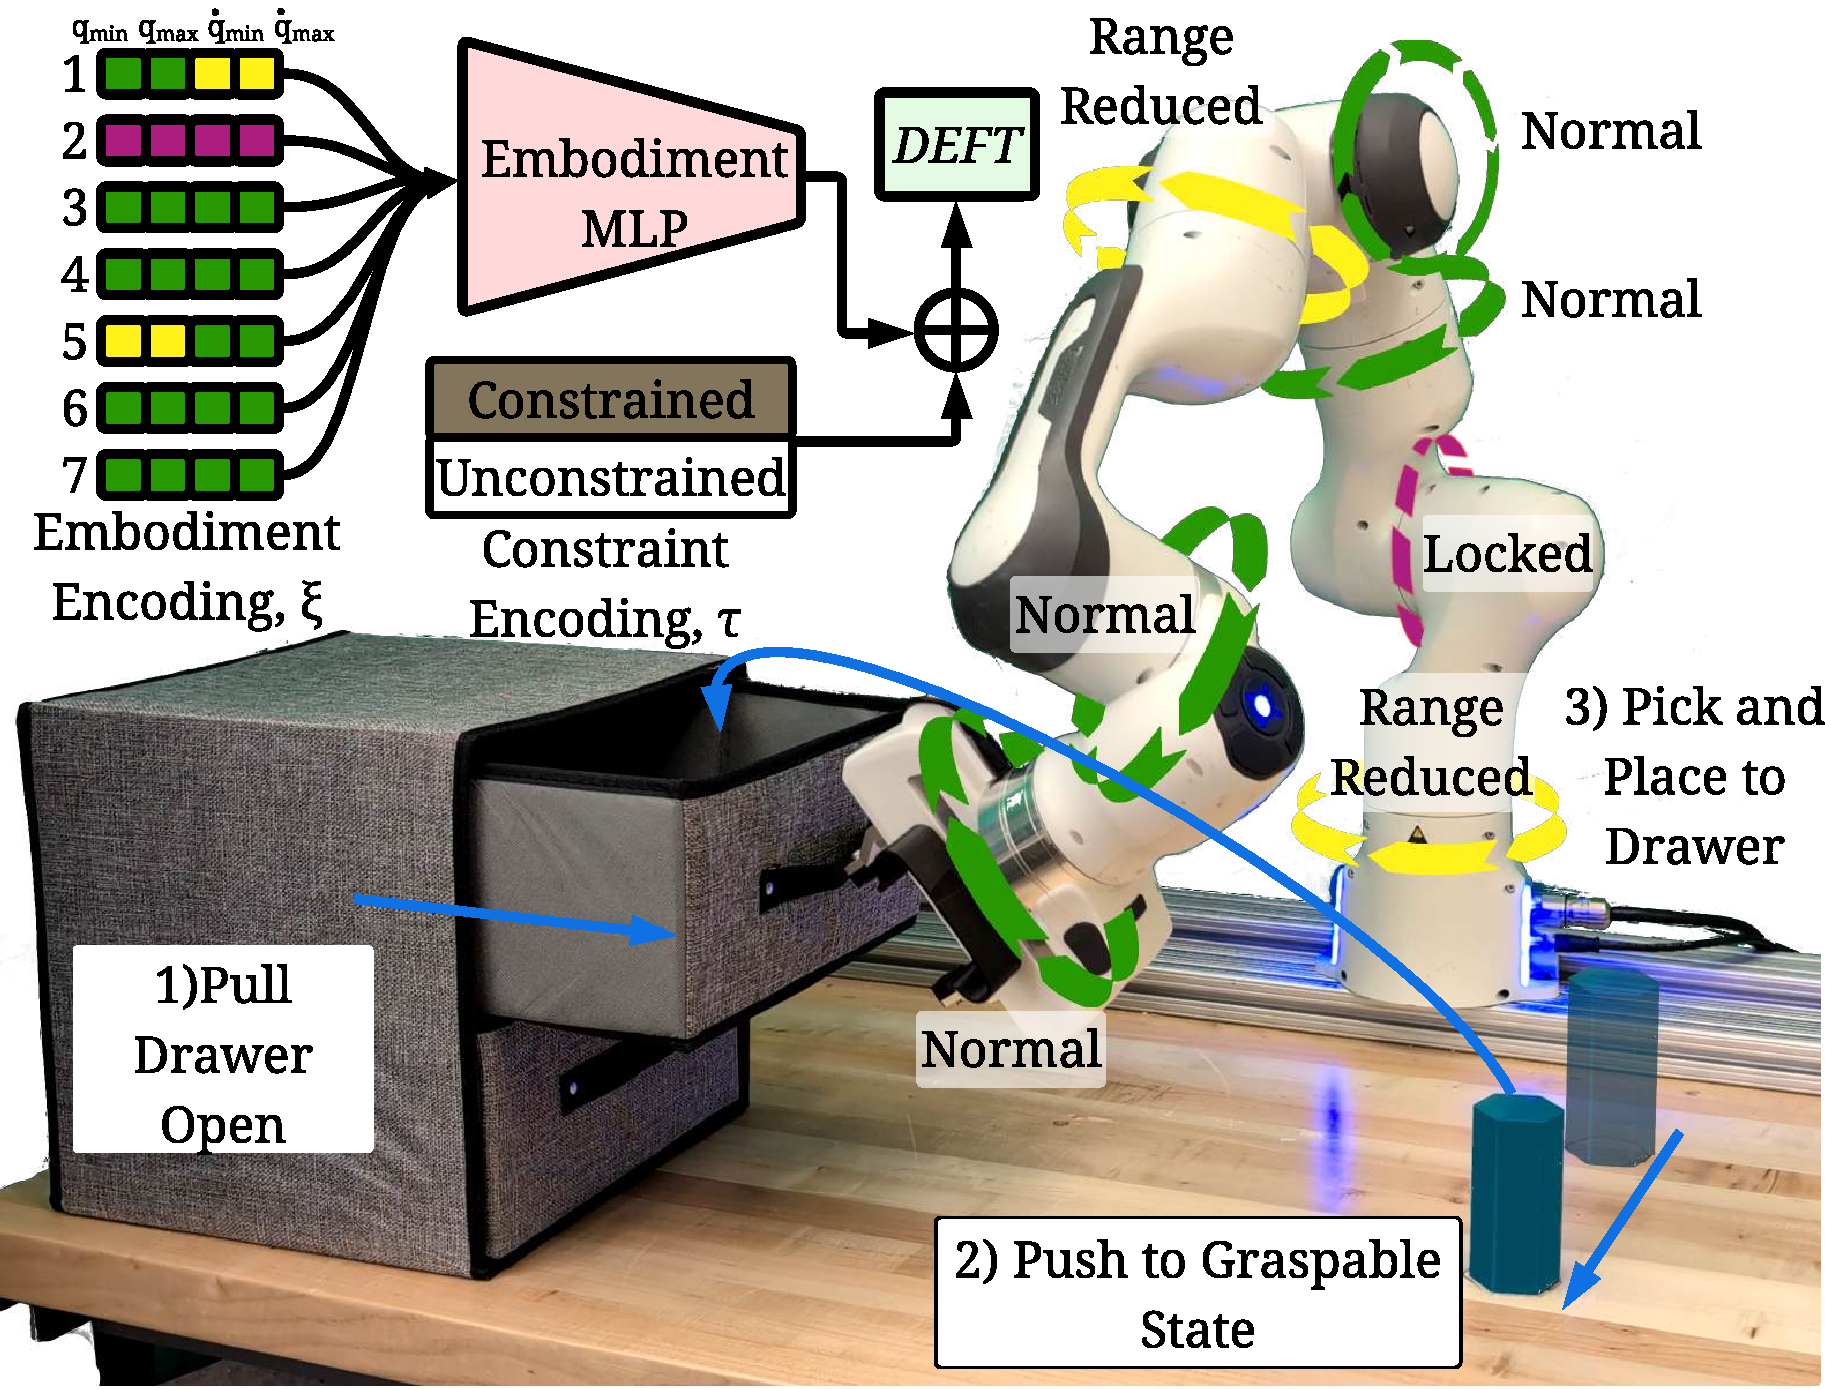
\includegraphics[width=\columnwidth]{../movingon/figures/first_page_figure_compressed.pdf}
    \caption{DEFT takes as input a structured embodiment encoding representing joint-level failures and a constraint encoding then synthesizes a feasible robot trajectory via a diffusion model. After experiencing a failure, a given task will likely need to be completed in a different manner. In this figure, the pick-and-place segment is no longer feasible, given the failure condition of a locked second joint and reduced velocity range on joint 1 and reduced angle range on joint 5, and the robot must now push the object to a graspable state to complete the task.}
    \label{fig:deft:first}
\end{figure}

\subsection{Embodiment-Aware Conditioning}
\label{sec:failures:conditioning}

To this end, we present \textit{DEFT}: a \textit{D}iffusion-based \textit{E}mbodiment-aware \textit{F}ail-active \textit{T}ask-conditioned trajectory generation framework, capable of maintaining robot manipulation functionality under failure conditions (\cref{fig:deft:first}). Our contributions are:
(i) an \textit{embodiment vector} encoding per-joint actuation failures for online adaptation to previously unseen failure-induced embodiments and
(ii) a \textit{constraint encoding} selecting between constrained and unconstrained motions to enable the use of multiple motion primitives.
Furthermore, we utilize start--goal inpainting and output clamping to enforce embodiment failure conditions \cite{repaint_lugmayr_2022}.

\begin{figure*}
  \centering
  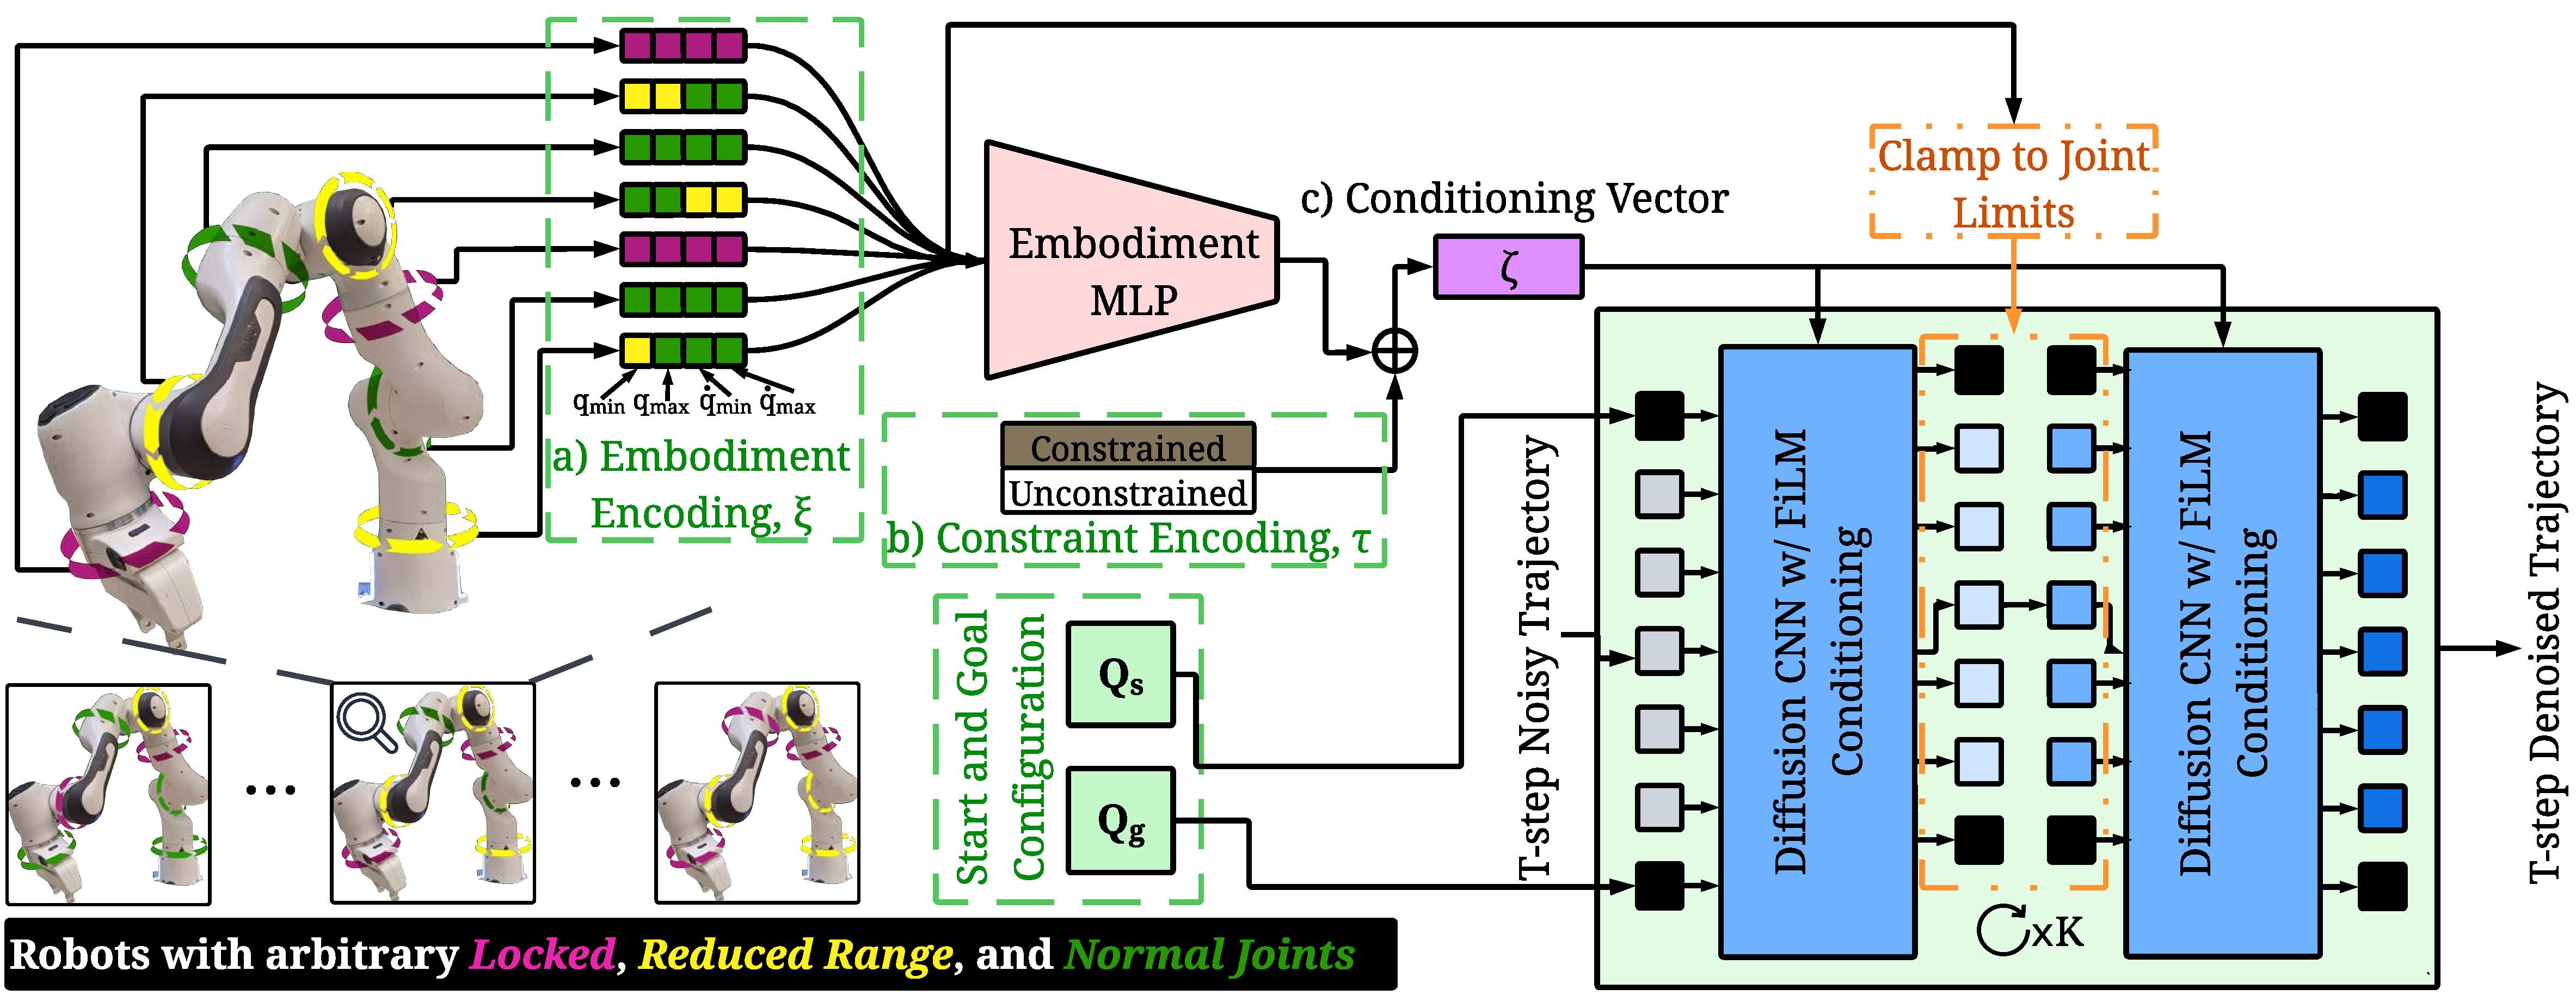
\includegraphics[width=\textwidth]{../movingon/figures/block_diagram.pdf}
  \caption{Overview of DEFT. (a) joint-level embodiment constraints are encoded into a structured representation capturing failure constrained joint position and velocity limits. This embodiment encoding is processed by a multilayer perceptron (MLP) and used to condition the diffusion model. (b) Task-specific constraints (e.g.\ unconstrained or constrained) are represented as one-hot vectors and concatenated with the embodiment encoding to constrain the generative process.
  Given these conditioning signals and start--goal joint configurations, the model generates feasible joint-space trajectories adapted explicitly to both the robot's degraded embodiment and task requirements. At each step of the denoising process the predicted joint values are clamped to the failure-induced robot joint limits.}
  \label{fig:deft:system}
\end{figure*}

Our goal is fail-active manipulation: generate functional, feasible trajectories under joint-level failures. We pose this as conditional trajectory generation given the failure-induced embodiment and the task constraint. Each failure specifies a new embodiment of the robot, and each constraint (e.g., \texttt{unconstrained} vs.\ \texttt{constrained} motion) induces a distinct trajectory distribution. Given the start and goal joint configurations the policy $\pi$ infers a future sequence of joint states over a fixed number of steps $T$. Unlike prior work that assumes a fixed set of failure configurations to control over, our method adapts online. It learns both the control behavior and the allowable motions from the current failure condition and the task constraint.

\paragraph{Embodiment Conditioning}
To inform the model of the robot's failure constrained embodiment, we use an embodiment encoding vector $\xi$ to condition the diffusion model. We model joint-level failures as per-joint constraints on the robot's actuation capabilities. Each failure embodiment is represented as $\xi = [\mathbf{e}_q, \mathbf{e}_{\dot{q}}] \in \mathbb{R}^{4N}$, with $\mathbf{e}_{q,j} = [q_j^{\min}, q_j^{\max}]^\top$ and $\mathbf{e}_{\dot{q},j} = [\dot{q}_j^{\min}, \dot{q}_j^{\max}]^\top$ for all $j \in \{1,\dots,N\}$ such that $\mathbf{0} \in \mathbf{e}_{\dot{q},j}$.
Failures reshape the robot's feasible configuration space and task-space reachability and exist in a continuous space, allowing $\xi$ to capture a wide spectrum of degradation severities, as shown in \cref{fig:deft:system}. Let $\{\mathbf{q}_t\}_{t=1}^T$ denote a trajectory over $T$ steps, where $\mathbf{q}_t \in \mathbb{R}^N$ is the joint configuration at time $t$, and $\dot{\mathbf{q}}_t$ its velocity. A configuration $\mathbf{q}_t$ satisfies the feasibility set $\mathcal{C}_t(\mathbf{q}_t,\xi)$ if:
\begin{equation}
\begin{aligned}
  \mathcal{C}_t(\mathbf{q}_t,\xi)=\Big\{\mathbf{q}_t\in\mathbb{R}^N\ \Big|\
  q_{t,j}\in \mathbf{e}_{q,j},\ \dot{q}_{t,j}\in \mathbf{e}_{\dot{q},j}\ \\ \ \forall j\in\{1,\dots,N\}\Big\}.
\end{aligned}
\end{equation}
A trajectory is feasible if $\mathbf{q}_{1:T}\in\bigcap_{t=1}^T \mathcal{C}_t(\mathbf{q}_t,\xi)$. We condition on failures structurally: the model learns to generate motion plans that obey the constraints.
To integrate embodiment information into the generative process, we pass $\xi$ through an MLP to produce an embedding that modulates the diffusion model via FiLM. To ensure that the trajectory connects the desired start and goal states we apply start--goal inpainting, fixing $(\mathbf{q}_s,\mathbf{q}_g)$ in the input trajectory. In addition, we clamp the trajectory to the limits during both training and inference.

\paragraph{Constraint Conditioning}
We further condition the model on discrete task constraints using a one-hot encoding vector, $\tau$. Let $\tau \in \{0,1\}^K$ be a one-hot vector with exactly one nonzero entry, such that
\[
\sum_{k=1}^{K} \tau_k = 1
\quad \text{and} \quad
\tau_k \in \{0,1\} \ \forall k.
\]
We concatenate $\tau$ with $\xi$ to form the conditioning vector $\zeta = [\xi, \tau]^\top$, which is injected via FiLM.
These constraints are not explicitly enforced during inference but must be learned implicitly through the conditioning signal. The constraint encoding also informs the model of task-imposed end effector constraints, which it otherwise would not know while operating in joint space.

\label{sec:failures:unified}
The formulation above enables zero-shot trajectory generation across diverse embodiments and task conditions. For example, when a shoulder joint becomes unusable, the robot can switch from lifting to pushing an object without task-specific retraining or policy switching.

We evaluate DEFT using two task constraints. \textit{Unconstrained} motion corresponds to a feasible trajectory between two points and includes unconstrained manipulation where the object is rigidly secured to the end-effector. \textit{Constrained} motion corresponds to planar, approximately straight-line motion with minimal end-effector orientation change---a spatial constraint for motion primitives such as pushing, pulling, or surface tracing. The valid trajectory sets are, respectively:
\begin{equation}
\begin{aligned}
  \mathcal{T}_\text{Unconstrained}=\Big\{\mathbf{q}_t \forall t\in\{1,\dots,T\}\ \Big|\
  & \mathbf{q}_1=\mathbf{q}_\text{s},\  \mathbf{q}_T=\mathbf{q}_\text{g},\ \\
  & \mathbf{q}_t\in \mathcal{C}_t(\mathbf{q},\xi)\Big\}.
\end{aligned}
\end{equation}
\begin{equation}
\begin{aligned}
  \mathcal{T}_\text{Constrained}
  = \Big\{\mathbf{q}_{t}\ \forall t\in\{1,\dots,T\}\ \Big|\ &
  \mathbf{p}_t\in\mathcal{P}\ \land\ \\ \Delta p_t\le \epsilon_p,
   \Delta \mathrm{R}_t\le \epsilon_R\ & \land\ \mathbf{q}_t\in \mathcal{C}_t(\mathbf{q},\xi)
  \Big\}.
\end{aligned}
\end{equation}

This allows \textsc{DEFT} to: 1) generalize to arbitrary failure configurations; 2) complete multiple manipulation primitives; and 3) handle multi-joint failures.

\subsection{Results}
\label{sec:failures:comparison}

We evaluate DEFT in two settings: (i) a \emph{simulation analysis} and (ii) a \emph{real-world comparison}. We ask if a single policy can remain \emph{fail-active} under embodiment degradation.

\paragraph{Simulation Analysis}
We test three hypotheses to probe DEFT's generalization to arbitrary joint failures (\textbf{H1} and \textbf{H2}) and to test whether DEFT produces both unconstrained and constrained motions (\textbf{H3}):
\begin{enumerate}
\item[\textbf{H.1}] Does DEFT obey embodiment constraints of arbitrary actuation failures more often than classical planners?
\item[\textbf{H.2}] Does DEFT \emph{generalize} to out-of-distribution (OOD) failures?
\item[\textbf{H.3}] Does DEFT adhere to constraint conditions more than approaches specialized to a single class of constraints?
\end{enumerate}

We use the motion planning method from data generation as our baseline, with RRT for \texttt{unconstrained} motions and differential IK with optimization for \texttt{constrained} motions. These baselines do not handle both primitives. In contrast, \textsc{DEFT} generates both within a unified model.

We evaluate on a fixed-base 7-DoF Franka Emika Panda arm. The study covers 4.7k failure conditions; of which 2.9k includes joint angle constraints (reduced and locked) and the rest are joint velocity constraints. For each condition, we randomly select 1--7 joints to be locked, range-limited, or velocity-restricted. Of these conditions, 22\% are in-domain (ID) and 78\% are out-of-domain (OOD). Each unique failure condition is tested 100 times, each with 100 start-goal pairs for a total of 4.7M trajectories evaluated.

\begin{table}[h]
\centering
\begin{tabular}{|c|c|c|c|}
\hline
\textbf{Hypothesis Summary} & \textbf{Test Condition}  & \textbf{Baseline} & \textbf{DEFT} \\ \hline
\textbf{H.1} Does DEFT handle & Angle Failure & 48.2\% & \textbf{84.3}\% \\ \cline{2-4}
arbitrary joint failures?& Velocity Failure & 32.5\% & \textbf{70.8}\% \\ \hline
\textbf{H.2} How well does DEFT & In Domain & \cellcolor{black} & \textbf{78.33\%} \\ \cline{2-4}
 handle unseen failures?& Out of Domain & \cellcolor{black} & \textbf{73.61\%} \\ \hline
\textbf{H.3} How well does DEFT  & Constrained & 30.93\% & \textbf{46.42}\% \\ \cline{2-4}
create multiple primitives?  & Unconstrained & 42.4\% & \textbf{99.58\%} \\ \hline
\end{tabular}
\caption{Success rate of the Baseline methods and the DEFT method.}
\label{tab:deft:performance}
\end{table}

\textsc{DEFT} consistently outperforms traditional planning baselines across various failure conditions (\cref{tab:deft:performance}). DEFT achieves a success rate of 74.51\% overall, while the baseline achieves only 36.85\%---an absolute improvement of 37.66 percentage points. Near-parity between ID and OOD success indicates DEFT extrapolates over joint space rather than memorizing seen cases. DEFT performs better for both primitives: 99.58\% vs.\ 42.40\% for unconstrained, and 46.42\% vs.\ 30.93\% for constrained motions.

\paragraph{Real-World Evaluation}

\begin{figure}
  \centering
  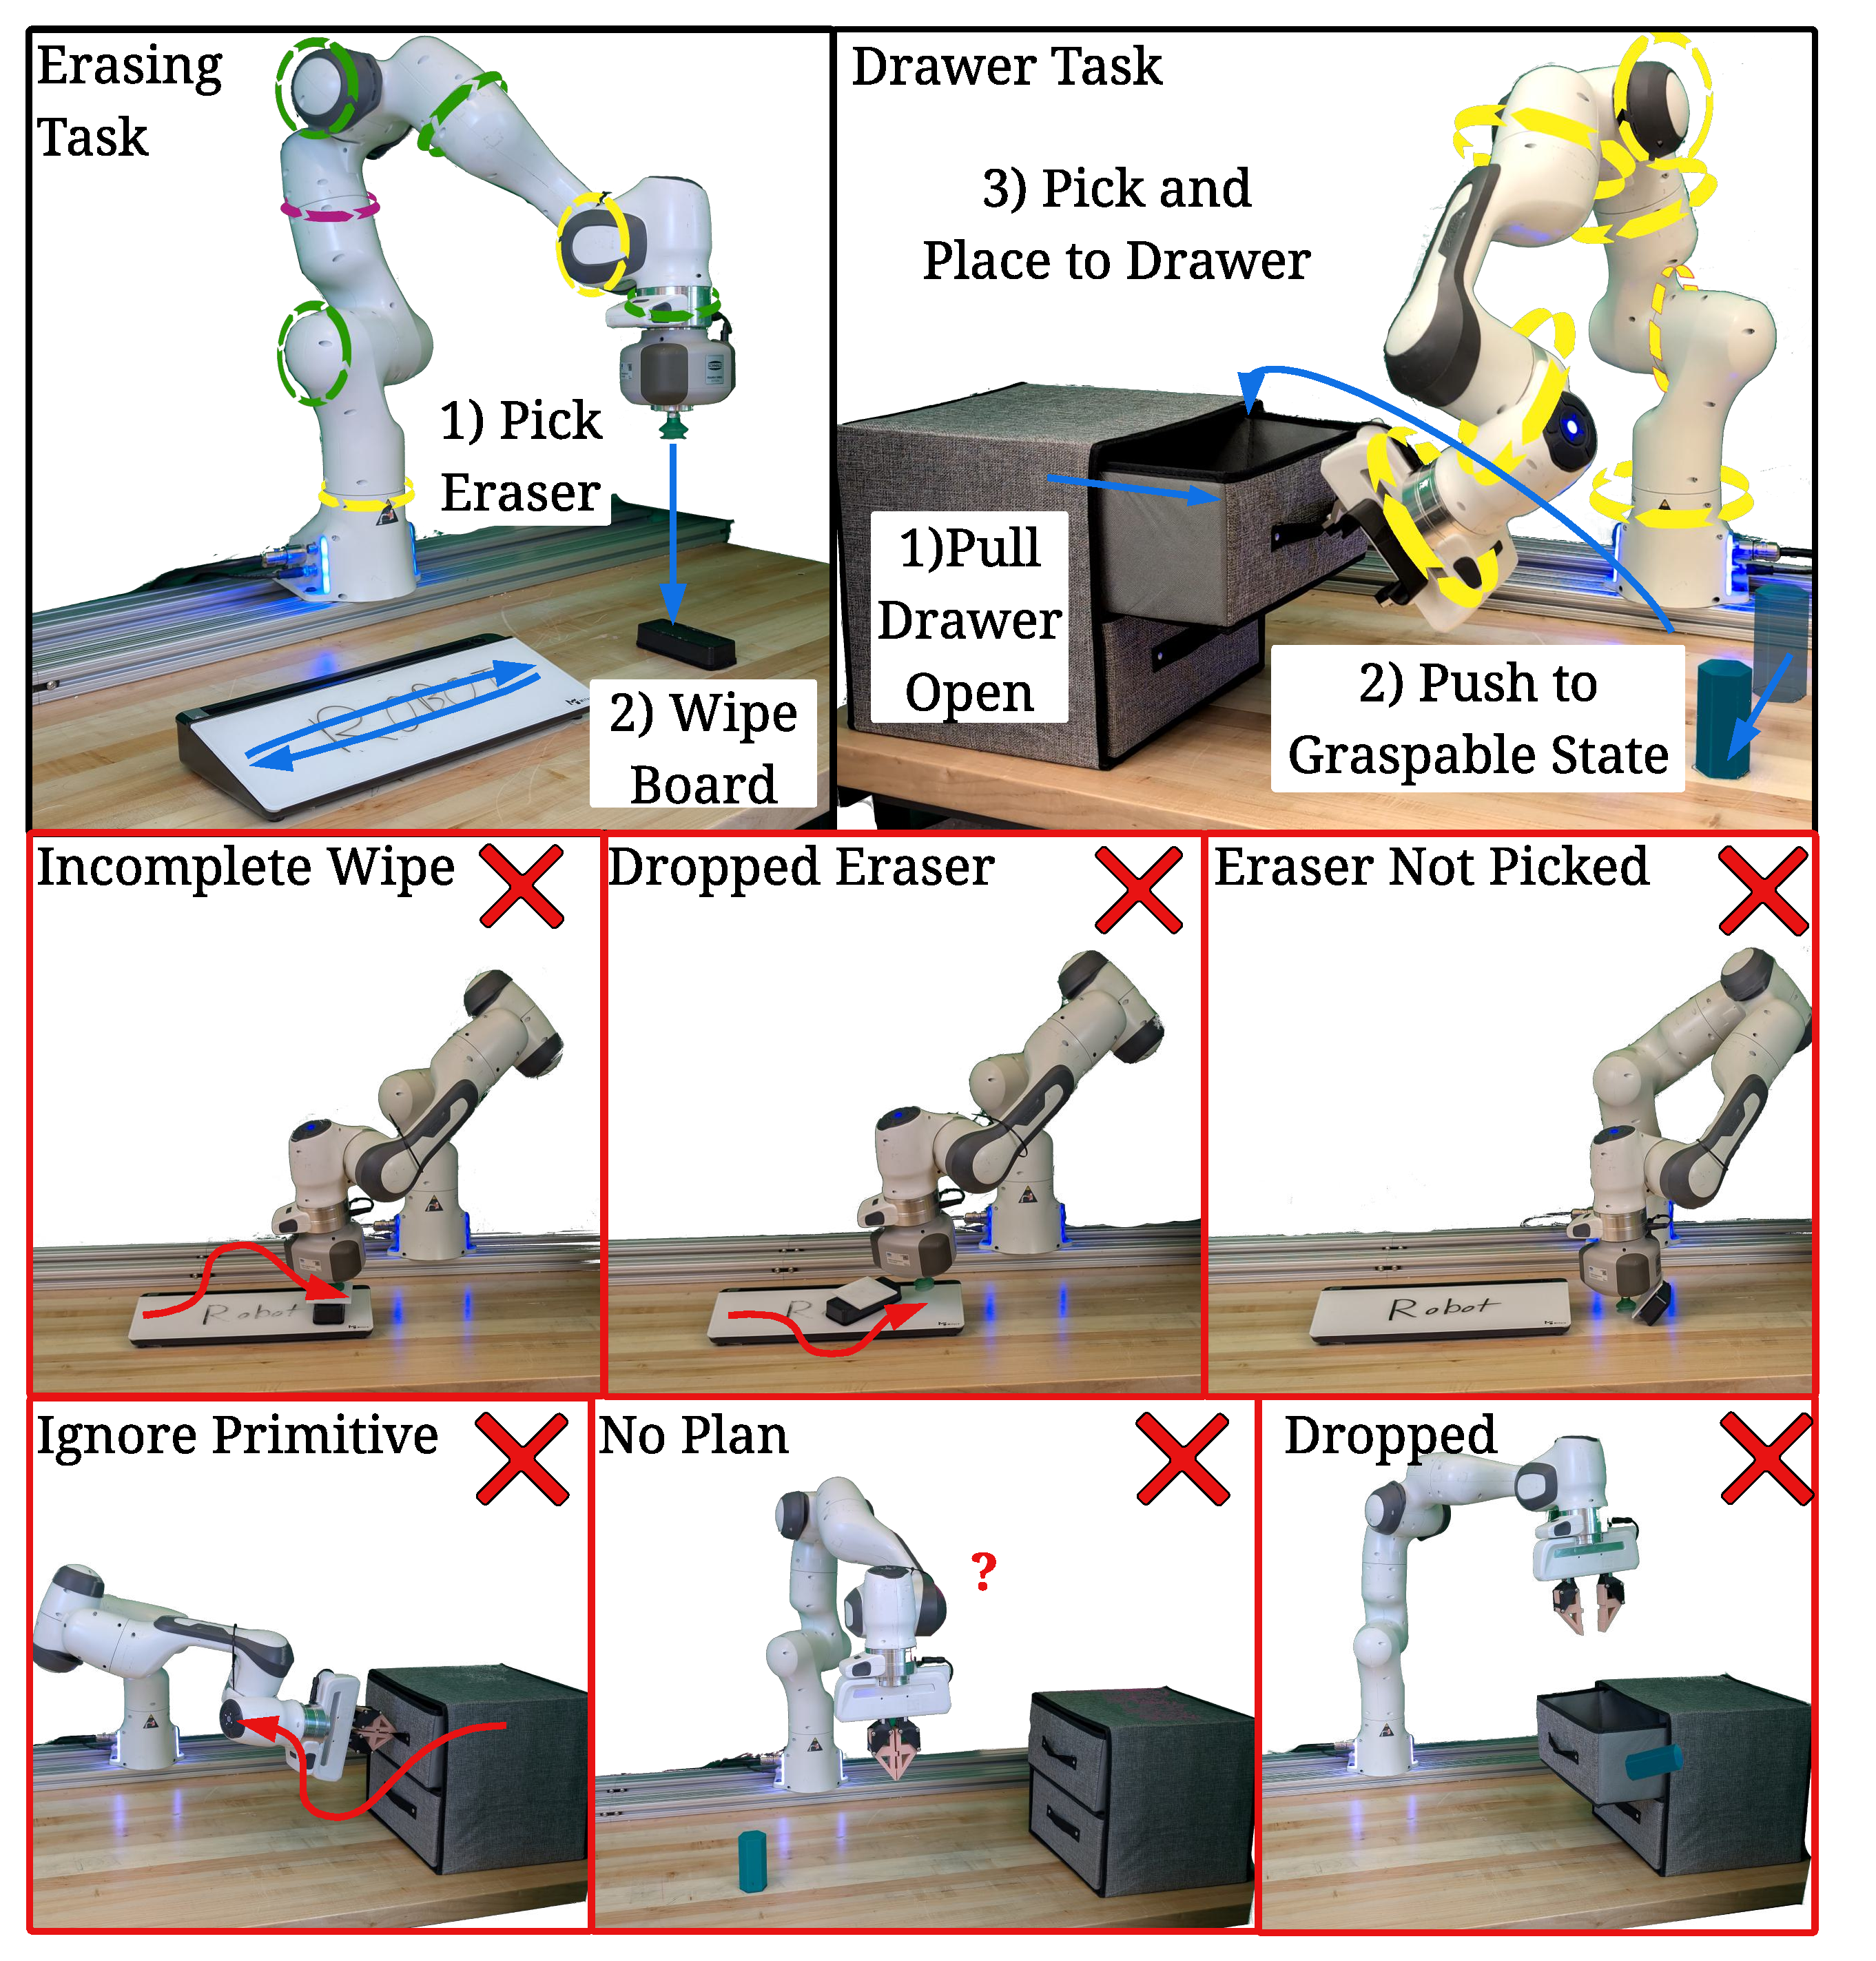
\includegraphics[width=\columnwidth]{../movingon/figures/real-task-explainer-vertical-compressed-1.pdf}
  \caption{Left (Erasing): The robot grasps an eraser from the table and performs back-and-forth sweeps to remove text. Right (Drawer): The robot opens a drawer, pushes an object to a graspable pose, places it inside, and closes the drawer.}
  \label{fig:deft:real}
\end{figure}

We test DEFT on two long-horizon, multi-primitive tasks (\cref{fig:deft:real}). The \textit{Drawer Task} consists of five sequential phases: pulling the drawer open, pushing the object to a graspable position, grasping, placing the object inside, and pushing the drawer closed. The \textit{Erasing Task} requires grasping an eraser from the table and sweeping it back and forth across a whiteboard to remove pre-written text. Together these tasks demand transitions between unconstrained free-space motion and constrained contact-rich interaction.

\begin{table}[h]
\centering
\caption{Real-world task results over 10 runs.}
\label{tab:deft:rw}
\begingroup
\setlength{\tabcolsep}{5pt}
\renewcommand{\arraystretch}{1.1}
\footnotesize
\begin{tabular}{@{}llcc@{}}
\hline
\textbf{Model} & \textbf{Task} & \textbf{Mean} & \textbf{Std.}  \\
\hline
DEFT                & Drawer  & \textbf{1.00} & 0.00  \\
DEFT                & Erasing & \textbf{1.00} & 0.00 \\
Optimization        & Drawer  & 0.00 & 0.00 \\
Optimization        & Erasing & 0.35 & 0.32 \\
DEFT-NoConditioning & Drawer  & 0.60 & 0.49 \\
DEFT-NoConditioning & Erasing & 0.93 & 0.12 \\
\hline
\end{tabular}
\endgroup
\end{table}

\textsc{DEFT} achieved perfect task completion on both real-world tasks (\cref{tab:deft:rw}). The Optimization baseline produced no executable plans on the drawer task. \textsc{DEFT}-NoConditioning succeeded in 6/10 drawer runs and 9.3/10 erasing runs, with failures attributable to missing embodiment conditioning and inpainting causing surface-constraint violations. These outcomes support our central hypothesis: embodiment and task conditioning, coupled with inpainting and clamping, yield a policy that remains fail-active under embodiment degradation.

Comparing against the sampling-based approach from Chapter~\ref{ch:constrained}, DEFT removes the need for pre-computation of kinodynamic action maps and generalizes to previously unseen failure conditions at inference time---directly addressing the computational demand limitation identified in that work. The cost is the loss of formal completeness guarantees, which sampling-based kinodynamic methods provide under certain conditions.

\section{What This Validates}
\label{sec:payload:validation}

This chapter establishes a principle that threads through the remainder of this thesis: \textit{dynamic constraints can be implicitly encoded into trajectory generation by conditioning on high-level object properties}.

Rather than explicitly checking torque feasibility at planning time---as the kinodynamic planner in \cref{ch:multiquery} must do---the diffusion model here learns the relationship between payload mass and the resulting joint torque constraints directly from data, internalizing this knowledge into its generative distribution.
A single scalar is sufficient to steer the denoising process toward trajectories that respect the full nonlinear complexity of the manipulator dynamics model across joint angle, velocity, and acceleration space simultaneously.
The result is constant-time generation that outperforms kinodynamic planners in both planning speed and success rate, at the cost of requiring feasible training trajectories.

This validates a broader generalization hypothesis: \textit{if a high-level object property governs the dynamic constraints a trajectory must satisfy, conditioning the generative model on that property is sufficient to implicitly respect those constraints.}
Payload mass is the simplest instantiation of this idea---a scalar that determines the end-effector wrench, which in turn determines joint torque feasibility throughout the workspace.
The case study above demonstrates a second instantiation: replacing the payload scalar with a structured embodiment vector encoding per-joint failure states yields a single model capable of fail-active behavior across an effectively unbounded space of failure conditions---again without explicit constraint checking at inference time.
